\title{Lab report on subject 001}
\author{
        John~O.~Woods,~Ph.D. \\
            \and
        Amie~E.~Hinds,~M.S. \\
            \and
        Luke Shafer,~M.S. \\
        R.~Daneel~Olivaw~Corporation\\
        908 Winston St., Suite \textsc{g} \\
        Houston, Texas 77009
}
\date{\today}

\documentclass[10pt]{article}

\usepackage{graphicx}

\begin{document}
\maketitle

%\begin{abstract}
%This is the paper's abstract \ldots
%\end{abstract}

\section{Objective}
Our contracted objective was to ascertain uses, if any, of subjects, which appear to be artifacts of some sort, and were found on certain near-earth asteroids.
Implicit in this objective is that damaging or removing components of these subjects must be avoided.

\section{Introduction}

All of the subjects appear to be of similar technological origin, having common components.
The purpose is unknown.
One possible taxonomy groups the subjects into two types based on the central component: mineral-based and glass-based.
However, we acknowledge that this taxonomy may highlight an arbitrary aspect of the subjects, and a separate taxonomy could be developed which emphasizes some other trait.
We therefore utilize this taxonomy, shown in Fig.~\figure{fig:taxonomy} and discussed below, solely for convenience.

%Subjects 001--004 and 007--008 consist of two parts, which we refer to as the mineral and the setting. Subjects 005--006 likewise have two components; however, in lieu of a mineral, the setting serves as a mount for what appears to be glass.

\subsection{Taxonomy}
The settings differ substantially between subjects 001--003, 004, and 007--008.
The settings in 001--003 consist of metal cut into geometric patterns, mounted on some type of what we surmise to be a connector.\footnote{We make the assumption that these are connectors on the basis of the oxidation on the pins.}
For 004, the setting consists of three metal dowels arranged in a triad.  
Whereas all of the other subjects were interpreted to be cut gemstones in metallic settings, subjects 005 and 006 appear to be hardware mounts for polished glass.
With 007 and 008, the 

\subsubsection{Terminology}

\textbf{Labyrinthine} describes the round plate-like settings. ADD DESCRIPTION HERE.
There is a layer of what may be either oxidation or some sort of protective coating; this layer appears to have been scraped off on the setting's edges and corners.

\section{Methods}
We endeavored to obtain as much information about the subjects as possible with as little potential impact on it as was feasible.

The mineral's properties may be categorized as either physical or optical.
We used a $10\times$ hand lens and ultraviolet light to discern basic physical properties.
For optical properties, a $45\times$ polarizing gemological microscope, a dichroscope, and a refractometer were employed.

\section{Results}

\subsection{Basic physical characteristics}
In subjects 001--004 and 007--008, the mineral appears to have been fashioned in a manner such that it resembles a gem.
Because of this observation, we have adopted some identifying methods and terms from gemology.

The mineral is yellow in color, transparent, and has a vitreous luster.
Unfortunately, certain diagnostic features such as cleavage and fracture were obliterated with the cutting and polishing by --- we presume --- the creators of this artifact.
Other physical properties such as hardness and specific gravity could not be tested due to our instructions not to abrade the subject.

\subsection{Optical characteristics}
Using the tools outlined above, we determined that the optical properties of the mineral are similar to those of quartz.
Specifically, we measured the refractive index (\textsc{ri}) to be exactly 1.55.
We used a polarizing microscope and determined that the mineral is anisotropic; the dichroscope allowed us to determine that the mineral is doubly refractive.

\subsection{Fundamental force irregularities}
While measurement of an object's mass seems so trivial as to belong in a grade-school lab report, our observations of the subject have led us to exercise a great deal of skepticism regarding the standard methods.
For example, a digital laboratory scale expresses its measurement in grams, which is a mass measurement --- but, in fact, the scale provides a measurement of force, not mass, and converts according to a calibration to the local gravitational field.

Several assumptions are implicit in such a measurement:
\begin{enumerate}
\item The object is subject only to gravitational force, and other forces (\textit{e.g.} magnetic) are tiny in comparison.
\item The object contains no regions that are of lower density than the atmosphere. Imagine, for example, a chamber containing helium at atmospheric pressure. Such a chamber would have an apparent weight less than that of an equivalent chamber containing standard atmosphere. Similarly, a chamber containing nothing --- a vacuum --- would weigh less than either the helium chamber or the atmosphere-containing chamber.
\item The object's temperature is at equilibrium with the environment (though this is only significant for gases and not solid objects, we mention it to be exhaustive in the face of confusing experimental results).
\end{enumerate}

Based on our observations, none of these assumptions necessarily apply.
Firstly, the subject produces a stronger than expected magnetic field based upon its apparent composition, and confusingly, the subject's dipole moment appears to rotate.
Not only does the dipole moment rotate, but it does so seemingly \textit{in tandem} with the placement of either a magnetometer or a simple compass relative to the artifact.

We next attempted to observe the weight of the subject, but found that the weight changed as we re-oriented the subject.
Indeed, when we cycled back through the orientations a second time, the apparent weight differed by up to around five percent from the first set of measurements.
When tested in the early afternoon, the scale recorded an average mass of 40.2 grams with a standard deviation of 1.2 grams.
We repeated the experiment an hour later and recorded an average mass of 41.5 grams --- again with a standard deviation of 1.2 grams.
Unfortunately, we were not allowed to keep the artifact any longer, which rather limited our ability to discern any meaningful trend.

However, one of us (Amie) noticed a peculiarity: the subject behaves extremely oddly when placed in a centrifuge.
We lacked the proper measurement tools, but observed that a 40-gram weight placed on the opposite end of a 0.25-meter centrifuge from the artifact produced a substantial imbalance.
We calculated a difference of roughly a tenth of a newton (order of magnitude, not exact) between the weight (mean) due to gravity and the weight due to centripetal acceleration.
It does not escape our notice that this odd behavior could actually allow the subject to be used as an energy source --- though further study is needed to determine whether the apparent weight correlates with the temperature.

We attempted to ascertain the volume of the device by placing it in a known volume of water and measuring the displacement.
Remarkably, despite apparently being made of materials significantly denser than water, it floated.
We next tried to use a straightened paperclip to push it down into the water, and measured a volume of around 100 ml.
However, the temperature of the paperclip increased rapidly, apparently through contact with the artifact. 
Indeed, Luke's fingers were burned.
We observed that the temperature of the water had increased substantially --- by nearly twenty degrees Celsius in under a minute (Fig.~\ref{fig:temperature}).
Further tests revealed the subject to be emitting broadly in the infrared.
Additionally, we found that the temperature increase was specific to the application of a downward force in water.
A downward force on a table produced no temperature change, nor did a sideways force in water --- though the temperature did increase when Luke inadvertently pushed slightly downward instead of sideways.
The temperature change did not appear to be sensitive to where we pushed (on the gem or the setting).
Again, it seems obvious that a device which rapidly produces so much heat when pushed underwater could serve as a rather simple and straightforward source of electricity; however, it is unclear where the energy for the temperature increase originates, and we prescribe several more weeks of testing.

\begin{figure}
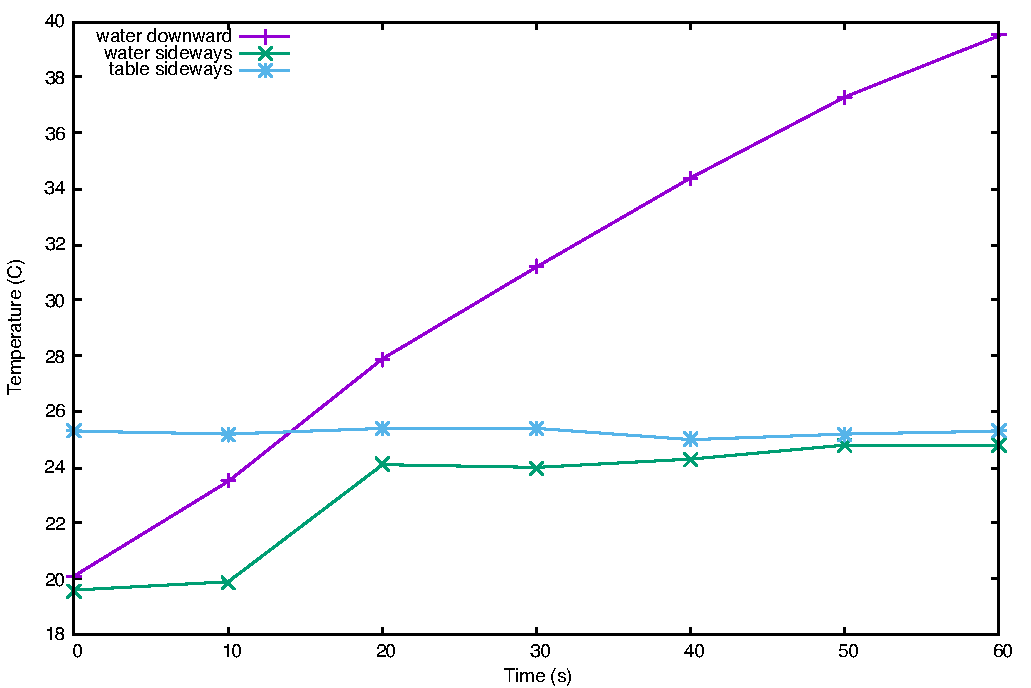
\includegraphics[width=1.0\textwidth]{01-temp.pdf}
\caption{\label{fig:temperature}\textbf{The application of downward force produces rapid temperature change in water.} A sideways force does not produce a change. The increase between 10 and 20 seconds on the `water sideways' time-points corresponds to inadvertent downward pressure. The `table sideways' plot temperature readings were taken with the temperature probe being used to push the subject, and thus reflect the subject temperature rather than water temperature.}
\end{figure}

\subsection{Radioactivity}
Our observations consistently showed the subject to be unremarkable in terms of its alpha, beta, and gamma emissions.

\section{Conclusions}\label{conclusions}
The subject responds unexpectedly to stimuli, based on its behavior in water and in the presence of a magnetometer.

The physical and optical properties of the mineral are consistent with those of lime citrine variety quartz.
Therefore, we believe it reasonable to consider other properties typically associated with quartz, which is known to have piezoelectric and pyroelectric properties.
These properties could help explain some of the unusual behaviors, such as the transmission of heat while submerged.
Given additional time, we recommend targeting investigations toward these properties.
 
The four hours of study we were permitted on the subject were insufficient for fully interrogating the range of possibilities produced by our testing, and the tests we performed have produced more questions than answers.

We urge extreme caution when transporting the subject due to its unpredictable behavior in a gravitational field.
It is unclear how the artifact would behave, for example, in orbit or on the way to orbit.\footnote{This type of information was not recorded when the subject was initially retrieved from 2000~\textsc{sg}344, the Aten asteroid where it was found. Frustratingly, the operators of the inbound re\"entry vehicle would not provide us with flight logs, arguing that the proprietary nature of their flight software and propulsion systems `regrettably' did not allow them to share those data.} Similarly, the rapid temperature increase could pose a serious fire hazard, and we lacked sufficient time to determine if submersion in other materials would also produce rapid heating.

%\bibliographystyle{abbrv}
%\bibliography{main}

\end{document}
This is never printed